\documentclass[letter, 10pt]{article}
\usepackage[utf8]{inputenc}
\usepackage[spanish]{babel}
\usepackage{amsfonts}
\usepackage{amsmath}
\usepackage[dvips]{graphicx}
\usepackage{url}
\usepackage[top=3cm,bottom=3cm,left=3.5cm,right=3.5cm,footskip=1.5cm,headheight=1.5cm,headsep=.5cm,textheight=3cm]{geometry}
\usepackage{listings}
\usepackage{color}

\begin{document}
\title{Computación Científica II\\ \begin{Large} Laboratorio \#1: Oscilador de
Duffing \end{Large}}
\author{
Rodrigo Fernández \\ 2673002-3 \\ \texttt{rfernand@inf.utfsm.cl} \and
Cristián Maureira \\ 2673030-9 \\ \texttt{cmaureir@inf.utfsm.cl} \and
Gabriel Zamora \\ 2673070-8 \\ \texttt{gzamora@inf.utfsm.cl} \and
Juan Pablo Cares \\ 2673066-K \\ \texttt{jcares@alumnos.inf.utfsm.cl} \and
Luiz Pizarro \\ 2673056-2 \\ \texttt{lupizarr@alumnos.inf.utfsm.cl} \and
Nicolas Ceroni \\ 2673028-7 \\ \texttt{nceroni@alumnos.inf.utfsm.cl}
}

\date{\today}
\maketitle

\section{Oscilador de Duffing}
El oscilador de Duffing es un ejemplo de un oscilador con excitación periódica y con un término no lineal de elasticidad, que viene dado por:

$$
	\ddot{x} + \delta \dot{x} + \beta x+ \alpha x^3 = \gamma \cos \omega dt
$$
\begin{itemize}
	\item Escriba la ecuación de Duffing en la forma $y = F (t, y)$.\\
	\textbf{Respuesta:}\\

	Sea  
	$$y_1 = x,$$
	$$y_2 = \dot{x}$$
	tenemos que 
	\begin{eqnarray}
	\dot{y_1} & = & \dot{x} \nonumber \\
	& = & y_2 \nonumber \\ \nonumber \\
	\dot{y_2} & = & \ddot{x} \nonumber \\
	& = & \gamma cos \omega t - \delta \dot{x} - \beta x - \alpha x^3 \nonumber \\
	& = & \gamma cos \omega t - \delta y_2 - \beta y_1 - \alpha {y_1}^3 \nonumber \\
	\nonumber
	\end{eqnarray}

Logrando así que:\\
$$
	\dot{y} = \begin{bmatrix} \dot{y_1} \\ \dot{y_2} \end{bmatrix} = \begin{bmatrix} y_2 \\ \gamma cos \omega t - \delta y_2 - \beta y_1 - \alpha {y_1}^3 \end{bmatrix} = \begin{bmatrix} F_1(t, y_1, y_2) \\ F_2(t, y_1, y_2) \end{bmatrix} = F(t,y) \nonumber
$$

además de que 
\begin{eqnarray}
	F_1(t, y_1, y_2) &=& y_2 \nonumber \\
	F_2(t, y_1, y_2) &=& \gamma cos \omega t - \delta \dot{y_1} - \beta y_1 - \alpha {y_1}^3 \nonumber \\
	y_1(t_0) &=& x(t_0) \nonumber \\
	y_2(t_0) &=& \dot{x}(t_0) \nonumber 
\end{eqnarray}

	\item Transforme el problema anterior en una ecuación integral de la forma:
$$
	y(t_n +1) = y(t_n - 1) + \int_{t_n-1}^{t_n+1} F(t, t(y))dt
$$
Escribiendo $y(t_k ) = y_k$ la ecuación queda:
$$
	y_{n+1} = y_{n-1} + \int_{t_n - 1}^{t_n +1} F(t,t(y))dt
$$
\end{itemize}

Aplicando la regla de Simpson para calcular la integral que aparece en
la ecuación integral, se obtiene la ecuación de recurrencias:

$$
y_{n+1} = y_{n-1} + \frac{h}{3} [F (t_{n-1} , y_{n-1} ) + F (t_n , y_n ) + F
(t_{n+1} , y_{n+1} )]
$$

\subsection{Programa con iteraciones de Newton para calcular $y_{n+1}$}
Antes de llegar y aplicar el programa, debemos hacer algunas aclaraciones y calculos antes:
La ecuación (4) define $y_{n+1}$ implícitamente en términos de $y_n$ ,
$y_{n-1}$. Notando que todas las expresiones y términos distintos de $y_{n+1}$
en (4) son conocidos, esta ecuación se reduce a una ecuación de la forma:
$$
y_{n+1}= \Phi(y_{n+1})
$$
En términos de sus componentes la ecuación (5) viene dada por:

$$
\Phi_1(u,v) = y_{n-1}^1+\frac{h}{3}(y_{n-1}^2+4y_{n}^2+v),
$$
$$
 \Phi_2(u,v) = y_{n-1}^2+\frac{h}{3}(\alpha [(y_{n-1}^1)^3+4(y_{n}^1)^3+u^3]+ \beta[y_{n-1}^1+4y_{n}^1+u]+\\ \delta[y_{n-1}^2+4y_{n}^2+v]-2 \gamma(2+cos(wh))cos(wt))
$$
\\\\
El problema consiste, entonces, en determinar un punto fijo $y_{n+1}$ de la función conocida $\Phi$, lo que en este ejercicio se propone hacerlo mediante iteraciones de Newton. Sean $u$, $v$, respectivamente, la primera y la segunda componente del vector incógnito $y_{n+1}$ y $\Phi_1$, $\Phi_2$ las funciones componentes de la función vectorial $\Phi$. Entonces (5) es equivalente al sistema de ecuaciones:

$$
\begin{Bmatrix} u=\phi_1(u,v) \\v=\phi_2(u,v) \end{Bmatrix}
$$

Queremos proceder por entera analogía al método de Newton unidimensional. Para ello escribiremos las ecuaciones (7) en la forma:

$$
z=z_1(u,v)=u- \phi_1(u,v),        z=z_2(u,v)=v- \phi_2(u,v)
$$


que representan dos superficies $S_1$ , $S_2$ en el espacio $\mathbb{R}^3$ . Las ecuaciones (7) corresponden a las curvas de nivel $\Gamma_1$, $\Gamma_2$, de nivel $z = 0$, de las superficies $S_1$, $S_2$ definidas por (7), esto es, $\Gamma_1$, $\Gamma_2$ son las curvas de intersección de las superficies $S_1$, $S_2$ con el plano coordenado $uv$ del espacio $\mathbb{R}^3$.

El problema consiste, entonces, en determinar el punto $(u^*, v^*)$ del
plano coordenado $uv$ donde las curvas $\Gamma_1$, $\Gamma_2$ se intersectan.
Con este propósito generaremos, mediante el método de Newton, una sucesión de
puntos $\{(u_\nu v_\nu )\}_{\nu \in{\mathbb{N}_0}}$ que se aproximan a $(u^*,
v^*)$ para $\nu\rightarrow{\infty}$.
Iniciamos las iteraciones de Newton con una aproximación $(u_0 ,v_0)$ de $(u^*, v^*)$, dada por:

$$
(u_0,v_0) := (y_n^1,y_n^2)
$$

Supongamos que ya hemos computado la aproximación $(u_\nu, v_\nu)$ de $(u^*,v^*)$. Si $z_1(u_\nu, v_\nu) = z_2 (u_\nu, v_\nu ) = 0$, o bien, en téminos computacionales, si:

$$
\left |{z_1(u_ \nu,v_\nu)}\right |< \varepsilon , \left |{z_2(u_ \nu,v_\nu)}\right |< \varepsilon 
$$

donde $0 < \epsilon << 1$ es un valor prescrito, entonces las iteraciones de Newton terminan y ponemos:

$$
y_{n+1}^1:=u_ \nu   ,  y_{n+1}^2:=v_ \nu
$$

Si, por el contrario, $z_1(u_\nu, v_\nu ) > \epsilon$, o bien $z_2(u_\nu , v_\nu ) > \epsilon$, entonces tenemos que continuar iterando con respecto a $\nu$. Para esos valores $u_\nu$ y $v_\nu$, se tiene:

$$
 z_1(u_ \nu,v_ \nu) = u_ \nu -  \phi_1(u_ \nu,v_ \nu) , z_2(u_ \nu,v_ \nu) = u_ \nu -  \phi_2(u_ \nu,v_ \nu)
$$

Razonando por analogía puesto que en el caso unidimensional de las iteraciones de Newton se considera la recta tangente a la curva $y = f (x)$ en el punto $x_k, f(x_k)$ y se determina el punto en que esa recta corta al eje x, en el caso bidimensional habrá que considerar los planos tangentes a las superficies $S_j : z = z_j(u,v)$ en los puntos $ u_\nu , v_\nu , z_j (u_\nu, v_\nu)\in{\mathbb{R}^3}$, para luego determinar las rectas $L_j$ de intersecció de estos planos con el plano $uv$. Si estas rectas no son paralelas, su punto de intersección determina los siguientes valores $(u_{\nu+1}, u_{\nu+1})$ para las iteraciones de Newton. Como se sabe, la ecuación de los planos tangentes aludidos vienen dadas por:

$$z-z_1(u_\nu,v_\nu) = \frac{{\partial z_1}}{{\partial u}}(u_\nu,v_\nu)(u-u_\nu)+\frac{{\partial z_1}}{{\partial v}}(u_\nu,v_\nu)(v-v_\nu)$$
$$z-z_2(u_\nu,v_\nu) = \frac{{\partial z_2}}{{\partial u}}(u_\nu,v_\nu)(u-u_\nu)+\frac{{\partial z_2}}{{\partial v}}(u_\nu,v_\nu)(v-v_\nu)$$

esto es, por:
$$
z-z_1(u_\nu,v_\nu) = (1-\frac{{\partial \phi_1}}{{\partial u}}(u_\nu,v_\nu))(u-u_\nu)+\frac{{\partial \phi_1}}{{\partial v}}(u_\nu,v_\nu)(v-v_\nu)
$$

$$
z-z_2(u_\nu,v_\nu) = -\frac{{\partial \phi_2}}{{\partial u}}(u_\nu,v_\nu)(u-u_\nu)+(1+\frac{{\partial \phi_2}}{{\partial v}})(u_\nu,v_\nu)(v-v_\nu)
$$

Las ecuaciones de las rectas $L_1$ y $L_2$ se obtienen haciendo $z = 0$ en las ecuaciones precedentes.
El sistema de ecuaciones resultantes se escribe en forma matricial como:

$$
\begin{bmatrix}{1-\frac{{\partial \phi_1 }}{{\partial u}}(u_ \nu,v_ \nu)
}&{-\frac{{\partial \phi_1 }}{{\partial v}}(u_ \nu,v_ \nu)}\\{-\frac{{\partial
\phi_2 }}{{\partial u}}(u_ \nu,v_ \nu)}&{1-\frac{{\partial \phi_2 }}{{\partial
v}}(u_ \nu,v_ \nu)}\end{bmatrix}\begin{bmatrix}{u-u_ \nu}\\{v-v_
\nu}\end{bmatrix}=\begin{bmatrix}{-z_1(u_ \nu,v_ \nu)}\\{-z_2(u_ \nu,v_
\nu)}\end{bmatrix}
$$
\\\\
La solución del sistema (15) para $u$, $v$ da la siguiente aproximación $(u_{\nu+1}, v_{\nu+1})$ de $(u^*, v^*)$:

$$
\begin{bmatrix}{u_{ \nu+1}}\\{v_{ \nu+1}}\end{bmatrix}=\begin{bmatrix}{u_
\nu}\\{v_ \nu}\end{bmatrix}+\begin{bmatrix}{1-\frac{{\partial \phi_1
}}{{\partial u}}(u_ \nu,v_ \nu)     }&{-\frac{{\partial \phi_1 }}{{\partial
v}}(u_ \nu,v_ \nu)}\\{-\frac{{\partial \phi_2 }}{{\partial u}}(u_ \nu,v_
\nu)}&{1-\frac{{\partial \phi_2 }}{{\partial v}}(u_ \nu,v_
\nu)}\end{bmatrix}^{-1} \begin{bmatrix}{-z_1(u_ \nu,v_ \nu)}\\{-z_2(u_ \nu,v_
\nu)}\end{bmatrix}
$$

\lstset{basicstyle=\footnotesize, breaklines=true, numbers=left,
frame=shadowbox, rulesepcolor=\color{black}}
\lstinputlisting{src/newton2.m}

\subsection{Iteraciones de Lipschitz}
\subsubsection{Estudio de la posibilidad de obtener $y_{n+1}$ con iteraciones de Lipschitz}
\input{src/2-estudio}
\subsubsection{Algoritmo para obtener $y_{n+1}$ con iteraciones de Lipschitz (en
matlab u Octave)}
\lstset{basicstyle=\footnotesize, breaklines=true, numbers=left,
frame=shadowbox, rulesepcolor=\color{black}}
\lstinputlisting{src/lipschitz.m}

\section{Análisis de los algoritmos}
\subsection{Descripción del algoritmo 1 (Newton)}
También conocido como \emph{Método de Newton-Raphson}.
Este método, es un de los más usados y efectivos que existen; en comparación a otros métodos,
el método de \emph{Newton-Raphson} no trabaja sobre un intervalo sino que basa su fórmula en un \emph{proceso iterativo}
al igual que el \emph{Método de Lipschitz o de iteración de punto fijo.}.

Para realizar una descripción del presente método,
supongamos que tenemos una aproximación $x_{i}$ a la raíz $x_{y}$,
de una función determinada $f(x)$,

\begin{center}
	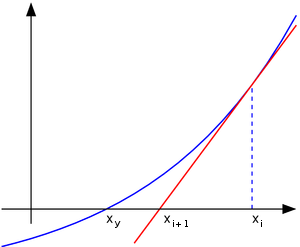
\includegraphics[width=150px]{img/newton}
\end{center}

Ahora si trazamos la recta tangente a la curva en el punto $(x_{i},f(x_{i}))$,
ésta va a cruzar el eje $x$ en un punto $x_{i+1}$,
que será nuestra siguiente aproximación a la raíz $x_{y}$.

Por otro lado, para calcular el punto $x_{i+1}$, calculamos primero la ecuación de la recta tangente.
Tenemos que la pendiente es:
$$m=f'(x_{i})$$
Por lo tanto la ecuación de la recta tangente a nuestra curva queda dada por:
$$y-f(x_{i}) = f'(x_{i})(x-x_{i})$$.

Ahora podemos asumir el valor de $y$, como $y=0$ y tenemos
$$-f(x_{i}) = f'(x_{i})(x-x_{i}),$$
despejando $x$, tenemos:
$$x=x_{i+1}=x_{i}-\frac{f(x_{i})}{f'(x_{i})},\ si\ f'(x_{i}) \neq 0$$

Como decíamos en un principio, el método de \emph{Newton-Raphson}  no trabaja con intervalos,
es decir, no tenemos la seguridad que encontraremos la raíz,
y de hecho no tenemos ninguna garantía de que nos aproximaremos a dicha raíz.

Como todo método, siempre existirán casos donde no converge a la raíz,
en cuyo caso se dice que el método diverge.
Sin embargo,
en los casos donde si converge a la raíz lo hace con una rapidez impresionante,
por lo cual es uno de los métodos preferidos por excelencia.

También es importante notar que en el caso de que $f'(x_{i}) = 0$,
el método no se puede aplicar.
De hecho, vemos geométricamente que esto significa que la recta tangente es horizontal
y por lo tanto no intersecta al eje $x$ en ningún punto,
a menos que coincida con éste, en cuyo caso $x_{i}$ mismo es una raíz de $f(x)$.

\subsection{Descripción del algoritmo 2 (Lipschitz)}
También llamado método de punto fijo, basado en uno de los resultados más importantes
del análisis matemático, el teorema del punto fijo de Banach, el cual dice
que:
\\
    Si en un espacio métrico $X$ completo tenemos una función de $X$ en $X$
contractiva, es decir, tal que existe $K<1$ tal que $d(f(x),f(y)) \leq
Kd(x,y)$
para cualesquiera $x$,$y\in X$, entonces existe un único punto fijo $x_0\in X$, es
decir, que satisface $f(x0) = x0$.
\\

Se trata de una herramienta básica en la prueba de la existencia de soluciones
de ecuaciones diferenciales. Otro de los usos de este resultado radica en el
análisis de sistemas dinámicos, que tiene numerosas aplicaciones, por ejemplo
en el estudio de modelos de población, modelos caóticos, etcétera. También es
importante en el estudio de métodos iterativos utilizados en el cálculo
numérico, por ejemplo en algunos problemas de ingeniería. Incluso determinados
fractales son puntos fijos de ciertas contracciones.\\

El método de punto fijo se aplica a una ecuación de la forma $g(x) =x$. Se
parte de una adivinanza inicial $x_0$ y se aplica la fórmula $x_{n+1}= g(x_n)$
para $n\geq 0$. En caso de que exista $\lim_{n \to \infty } x_n = p$, si $g$
es continua en este valor $p$, se tiene que
\begin{displaymath}p=\lim_{n \to \infty } x_n = \lim_{n \to \infty }
g(x_{n-1}) = g(\lim_{n \to \infty } x_{n-1} ) = g(p) \end{displaymath}


De esta forma, $p$ sería una solución buscada. 

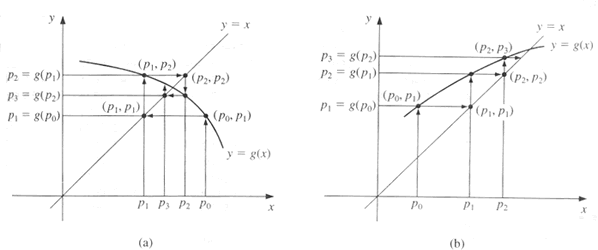
\includegraphics[width=400px]{img/PuntoFijo}

El siguiente teorema nos da algunas condiciones suficientes para
la convergencia del algoritmo de punto fijo para un valor inicial escogido en
un intervalo apropiado:

Sea $g(x)$ una función continua en un intervalo $[a, b]$ tal que
$g(x) \in [a,b] \; \; \forall x \in [a,b]$, entonces $g(x)$, tiene un punto
fijo $p$ en $[a, b]$ .

Si además, $g^\prime (x) $ existe en $]a,b[$ y es posible hallar una constante
$k<1$ tal que $g^\prime (x) \leq k, \; \mbox{para todo } x \in ]a,b[$,
entonces el punto fijo de $g(x)$en $[a, b]$ es único.

Adicionalmente, si $g^\prime (x) $ es continua en $]a,b[$ y $g^\prime (p) \neq
0$, entonces para cualquier valor inicial $x_0 \in [a, b]$, la sucesión
definida por
\begin{displaymath}x_{n+1}=g(x_n)\end{displaymath}
 
converge a $p$ y $\vert x_{n+1}-p\vert<k\vert x_n-p\vert$

\subsection{Resultados de los algoritmos}
Luego de programar los algoritmos en matlab se procedió,
a ejecutarlos para ver los resultados, y notar si se existía un
valor parecido en ambas situaciones.

\begin{tabular}{llcll}
	\textbf{Newton:} & $y_{n+1} = {-0.8159 \brack -0.3694}$ & &\textbf{Lipschitz:} & $y_{n+1} = {-0.8133 \brack -0.3703}$ \\
\end{tabular}

Con respecto al tiempo que se empleo en realizar el cálculo
de cada algoritmo, nos dimos cuenta que no siempre era el mismo,
esto tiene completa relacion porque no realizamos los cálculos
en una máquina \emph{Real Time}, por lo tanto lo que decidimos
fue poder realizar 10 ejecuciones y promediar un valor,
para poder obtener un valor cercano al real.

A continuación se muestra una tabla con los tiempos (en segundos) 
que resultaron de las 10 ejecuciones de nuestros algoritmos.
\begin{center}
\begin{tabular}{|c|c|c|c|c|c|c|c|c|c|c|c|}
	\hline
	Método & 1 & 2 & 3 & 4 & 5 & 6 & 7 & 8 & 9 & 10  \\\hline 
	Lipschitz (s) & 25.15 & 21.46 & 21.03 & 23.00 & 23.63 & 23.59 & 22.69 & 21.83 & 25.18 & 24.04  \\\hline
	Newton (s)    & 23.85 & 23.66 & 23.23 & 21.50 & 21.45 & 22.47 & 23.25 & 22.36 & 24.33 & 21.83  \\\hline
\end{tabular}
\end{center}
Finalmente tenemos el promedio:
\begin{tabular}{llcll}
	\textbf{Newton:} & 22.793 segundos & &\textbf{Lipschitz:} & 23.160 segundos \\
\end{tabular}

\subsection{Comparativas}

\scriptsize
\begin{tabular}[b]{|l|l|l|}
\hline
a	&	\textbf{Newton}	&	\textbf{Lipschitz}	\\
\hline
0	&	for n=1 a N	&	lo mismo \\
1	&	hace $t_{n+1} = t_n +h$	& lo mismo	\\
2	& $\Phi_k = \Phi_k (u,v)$	& lo mismo	\\
3	& $z_1(u, v) = u - \Phi_1 (u,v)$	& lo mismo	\\
4	& $z_2(u, v) = u - \Phi_2 (u,v)$	& lo mismo	\\
5	& $v = 0; (u_0, v_0) = (y^1_n, y^2_n);$	& lo mismo	\\
6	& while $|z_1(u_v, v_v)| > \epsilon$ or $|z_2(u_v,v_v) |> \epsilon)$ & lo mismo	\\
7	& $ \left[ {\begin{array}{c} u_{v+1}  \\ v_{v+1}\\ \end{array} }\right]  = 
\left[ {\begin{array}{c} u_{v}  \\ v_{v}\\ \end{array} }\right]  +
\left[ {\begin{array}{cc} 1-\frac{\delta \Phi_{1}}{\delta u} (u_{v}, v_{v}) & -\frac{\delta \Phi_{1}}{\delta v} (u_{v}, v_{v})   \\
 -\frac{\delta \Phi_{1}}{\delta u} (u_{v}, v_{v})  & 1-\frac{\delta \Phi_{2}}{\delta
v} (u_{v}, v_{v}) \\ \end{array} }\right]^{-1}
 \left[ {\begin{array}{c} -z_{1} (u_{v}, v_{v})  \\ -z_2 (u_{v}, v_{v})\\ \end{array} }\right] 
$ & $u_{v+1} = \Phi_1 (u_{v}, v_{v}); v_{v+1} = \Phi_2 (u_v, v_v);$	\\
8	& $v = v+1$ & lo mismo	\\
9	& end while & lo mismo	\\
10	& $(y^1_n , y^1_n+1) = (u_v, v_v)$ & lo mismo	\\
11	& end for & lo mismo	\\
\hline
\end{tabular}
\\
\normalsize


Claramente podemos observar que las diferencias radican en el tipo de
resolución, en el cual el algoritmo con iteraciones de Lipschitz es más simple
que realizar las iteraciones de Newton.

La cantidad de operaciones que realiza una iteración de Lipschitz quedan
definidas por resolver $\Phi_1 (x,y)$ y $\Phi_2 (x,y)$. En cambio, una
iteración de Newton en este caso debe calcular el plano tangente respectivo a
cada función $y$ ($y_1$ e $y_2$), y luego resolver el intercepto con el plano
del eje $X$ para obtener las soluciones de la ecuación que utiliza para ir
acercándose al valor de $y_{n+1}$.

Ahora, el método de Lipschitz, a pesar de ser más simple, requiere de muchas
más iteraciones que el método de Newton, lo cual aumenta el tiempo de
resolución del problema en \textbf{inserte valor acá}, a lo cual si uno le suma la
poca capacidad de paralelización en la resolución del problema, puede llegar a
ser más costosa computacionalmente. 
\\
Otra diferencia fundamental de estos dos métodos, es que para poder utilizar
el método iterativo de Lipschitz, primero hay que verificar que la función
converja de la siguiente forma:\\
Dado $y'=f(x,y)$, despejamos $f(x,y)$ para lograr que en un costado de la
ecuación quede solamente $x$ y la igualamos a $x=g(x,y)$
\begin{itemize}
	\item Si $|g'(x,y)|< 1$ Converge linealmente
	\item Si $|g'(x,y)|= 0$ Converge cuadraticamente.
	\item Si $|g'(x,y)|> 1$ Diverge linealmente
\end{itemize}

Si la condición de convergencia no se cumple, simplemente no podríamos
utilizar este método para resolver el problema, ya que nos quedaríamos iterando
infitamente, alejándonos cada vez más de la solución.

\subsection{Conclusiones}
Antes definamos Velocidad de convergencia 
La velocidad de convergencia de un método  iterativo está dada por el número de  iteraciones que son
necesarias  para  alcanzar  un  cierto  grado  de  exactitud.  Puesto  que  es  muy  difícil  obtener  valores
absolutos  de  velocidad  de  convergencia,  los  distintos métodos  se  suelen  encasillar  por  su  orden  de
convergencia.

Sea $e_{n+1}$ el error que se tiene en la determinación de la raíz en la iteración $n+1$

$$e_{n+1}=x_{n+1}-x^*$$

Se define un Algoritmo iterativo de orden $m$ como aquel que cumple

$$ \displaystyle\lim_{x \to\infty}{\frac{\left |{x_{n+1} - x^*}\right |}{\left |{x_n - x^*}\right |^m}} = \displaystyle\lim_{x \to\infty}{\frac{\left |{e_{n+1}}\right |^m}{\left |{e_n}\right |}}  = K_m $$

en donde $K_m$ es una constante llamada error asintótico. En general se tiene convergencia lineal si $m = 1$ y convergencia cuadrática si $m = 2$.
Otra forma de interpretar el límite es diciendo que para n “suficientemente grande”,

$$ \left |{e_{n+1}}\right | = K_m \left |{e_n}\right |^m $$

Puesto que para valores grandes de $n$, en es un número pequeño, la velocidad de convergencia crece exponencialmente con el orden de convergencia. Por lo que es deseable un orden alto de convergencia.
Veamos el orden de convergencia del método de iteraciones de punto fijo o Lipschitz. Para ello debemos calcular la dependencia que existe entre $e_{n+1}$ y $e_n$. Usemos el desarrollo por series de Taylor de la siguiente manera:

$$ e_{n+1} \\ =  x_{n+1} - \alpha \\ =  \varphi(x_n) -  \varphi(\alpha ) \\ =  \varphi(\alpha )+ \varphi'(\alpha )(x_n - \alpha )+\frac{1}{2} \varphi''(\alpha+ \theta e_n)e_n^2 -  \varphi(\alpha ) \\ =  \varphi'(\alpha )(x_n-\alpha )+\frac{1}{2} \varphi''(\alpha +  \theta e_n)e_n^2 $$

Observemos en la última igualdad que, a menos que $ \varphi'(\alpha) = 0 $, el algoritmo de las iteraciones sucesivas
converge linealmente a la solución. Por otra parte, obtenemos la condición de convergencia cuadrática del método que es, $ \varphi'(\alpha) = 0 $.
\\\\
Una ventaja del método de Lipschitz consiste en su gran sencillez y flexibilidad para elegir la forma de $ \varphi'(\alpha)$. Sin embargo, es muy importante la formación de la función $ \varphi'(\alpha) $ en la ecuación $ x = \varphi'(\alpha)$; de las múltiples opciones que pueden existir, ya que no siempre converge con cualquier forma elegida de $ \varphi'(\alpha) $.
\\\\
De la misma manera se puede obtener que la velocidad de convergencia del metodo de Newton Raphson es del orden 2 y el error absoluto entre la aproximación actual y la aproximación anterior es proporcional al cuadrado del error calculado en la anterior iteración, por lo cual pude afirmarse que cada iteración duplica el número de dígitos correctos en la aproximación, lo que hace que este metodo sea mas eficiente que las iteraciones de Lipschitz (que es de orden lineal), por estas razones es que es un algoritmo altamente utilizado. Pero, a pesar de que el método de Newton Raphson es muy eficiente, hay situaciones donde se comporta de manera deficiente.






\end{document}
